\documentclass[aspectratio=169]{beamer}

% --- Generate BibTeX file automatically (same mechanism as the template) ---
\usepackage{filecontents}
\begin{filecontents}[overwrite]{references.bib}
@InProceedings{sun2024diversity,
  title={On the Diversity and Realism of Distilled Dataset: An Efficient Dataset Distillation Paradigm},
  author={Sun, Peng and Shi, Bei and Yu, Daiwei and Lin, Tao},
  booktitle={Proceedings of the IEEE/CVF Conference on Computer Vision and Pattern Recognition (CVPR)},
  year={2024}
}

@article{wang2018dataset,
  title={Dataset Distillation},
  author={Wang, Tongzhou and Zhu, Jun-Yan and Torralba, Antonio and Efros, Alexei A},
  journal={arXiv preprint arXiv:1811.10959},
  year={2018}
}

@inproceedings{yin2023squeeze,
  title={Squeeze, Recover and Relabel: Dataset Condensation at ImageNet Scale From A New Perspective},
  author={Yin, Zeyuan and Xing, Eric and Shen, Zhiqiang},
  booktitle={Thirty-seventh Conference on Neural Information Processing Systems},
  year={2023}
}

@article{papyan2020prevalence,
  title={Prevalence of neural collapse during the terminal phase of deep learning training},
  author={Papyan, Vardan and Han, X. Y. and Donoho, David L.},
  journal={Proceedings of the National Academy of Sciences},
  volume={117}, number={40}, pages={24652--24663}, year={2020}
}

@inproceedings{chen2018fast,
  title={Fast Greedy MAP Inference for Determinantal Point Process to Improve Recommendation Diversity},
  author={Chen, Laming and Zhang, Guoxin and Zhou, Eric},
  booktitle={Advances in Neural Information Processing Systems (NeurIPS)},
  year={2018}
}

@inproceedings{guo2017calibration,
  title={On Calibration of Modern Neural Networks},
  author={Guo, Chuan and Pleiss, Geoff and Sun, Yu and Weinberger, Kilian Q.},
  booktitle={International Conference on Machine Learning (ICML)},
  year={2017}
}

@inproceedings{hendrycks2017baseline,
  title={A Baseline for Detecting Misclassified and Out-of-Distribution Examples in Neural Networks},
  author={Hendrycks, Dan and Gimpel, Kevin},
  booktitle={International Conference on Learning Representations (ICLR)},
  year={2017}
}

@inproceedings{liu2020energy,
  title={Energy-based Out-of-distribution Detection},
  author={Liu, Weitang and Wang, Xiaoyun and Owens, John D. and Li, Yixuan},
  booktitle={Advances in Neural Information Processing Systems (NeurIPS)},
  year={2020}
}

@inproceedings{lee2018simple,
  title={A Simple Unified Framework for Detecting Out-of-Distribution Samples and Adversarial Attacks},
  author={Lee, Kimin and Lee, Kibok and Lee, Honglak and Shin, Jinwoo},
  booktitle={Advances in Neural Information Processing Systems (NeurIPS)},
  year={2018}
}
\end{filecontents}

% Encoding and fonts (mirrors the template: inputenc left off on purpose)
\usepackage[T1]{fontenc}
% \usepackage[utf8]{inputenc}

% Core packages
\usepackage{hyperref}
\usepackage{amsmath, amssymb, latexsym}
\usepackage{graphicx}
\usepackage{xcolor}
\usepackage{booktabs}
\usepackage{listings}
\usepackage{adjustbox}
\usepackage{caption}

% Citation styling
\usepackage[square,numbers]{natbib}
\bibliographystyle{unsrtnat}

% Metadata
\title{Trustworthy Dataset Distillation\\ via Variance-Aware Crop Selection}
\subtitle{A trustworthiness study of RDED}
\author{Nikolaos Andriotis}
\institute{Aristotle University of Thessaloniki}
\date{\today}

\begin{document}

% --- Title slide ---
\begin{frame}
    \titlepage
\end{frame}

% --- Outline ---
\begin{frame}{Outline}
    {
    \footnotesize
    \renewcommand{\baselinestretch}{0.85}
    \tableofcontents[hideallsubsections]
    }
\end{frame}

% ==========================================
\section{Background \& Motivation}
% ==========================================

\begin{frame}{RDED: optimization-free dataset distillation \cite{sun2024diversity}}
    \begin{columns}
        \begin{column}{0.92\textwidth}
            \centering
            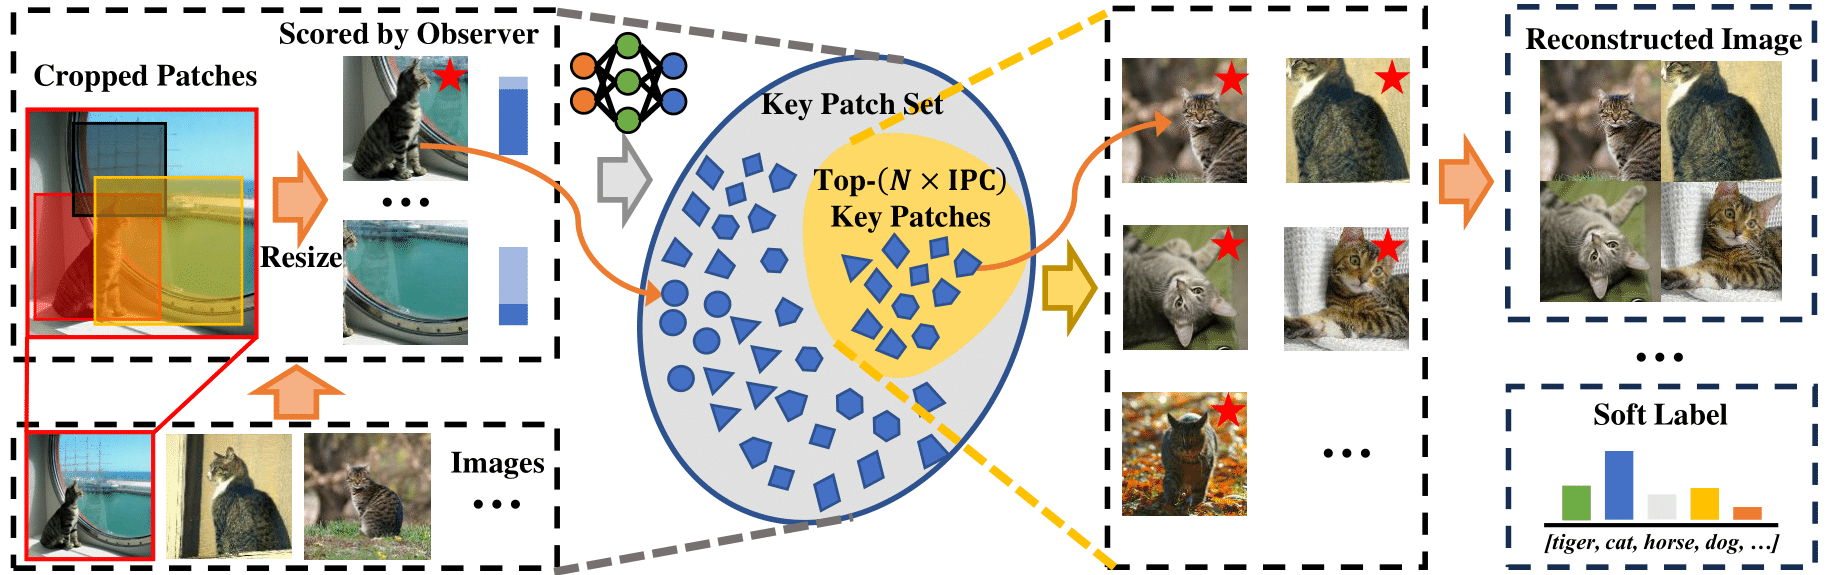
\includegraphics[width=0.9\linewidth,height=0.40\textheight,keepaspectratio]{figures/framework.png}
        \end{column}
    \end{columns}

    \vspace{1.0cm}
    {\scriptsize
    \textbf{Pipeline (per class):} crop real images $\to$ score each crop with a \emph{frozen} teacher
    ($\ell_j=-\log\operatorname{softmax}(z_j)_{[y]}$) $\to$ keep the most-confident crops $\to$ stitch into
    IPC images/class $\to$ \textbf{relabel} with the teacher's soft labels. A \textbf{student} is trained
    \emph{only} on this set by knowledge distillation.}

\end{frame}

% ==========================================
\section{Trustworthiness Diagnostic}
% ==========================================

\begin{frame}{Diagnostic overview --- student vs.\ teacher (full grid)}
    \centering
    \resizebox{0.6\linewidth}{!}{
        \renewcommand{\arraystretch}{1.15}
        \setlength{\tabcolsep}{6pt}
        \begin{tabular}{l c cc cc cc cc}
            \toprule
            & & \multicolumn{2}{c}{\textbf{top-1}} & \multicolumn{2}{c}{\textbf{ECE}}
              & \multicolumn{2}{c}{\textbf{AUROC}} & \multicolumn{2}{c}{\textbf{OSCR}} \\
            \cmidrule(lr){3-4}\cmidrule(lr){5-6}\cmidrule(lr){7-8}\cmidrule(lr){9-10}
            \textbf{cell} & \textbf{IPC} & S & T & S & T & S & T & S & T \\
            \midrule
            C100/Conv3 & 1  & 21.6 & 59.7 & .203 & .104 & .647 & .946 & .169 & .577 \\
                       & 10 & 48.6 & 59.7 & .097 & .104 & .903 & .946 & .457 & .577 \\
                       & 50 & 57.5 & 59.7 & .097 & .104 & .928 & .946 & .549 & .577 \\
            \midrule
            C100/RN18  & 1  & 11.2 & 70.9 & .274 & .122 & \textbf{.379} & .946 & .059 & .690 \\
                       & 10 & 44.7 & 70.9 & .190 & .122 & .765 & .946 & .391 & .690 \\
                       & 50 & 63.3 & 70.9 & .132 & .122 & .894 & .946 & .594 & .690 \\
            \midrule
            Tiny/Conv4 & 1  & 13.3 & 50.2 & .177 & .065 & \textbf{.423} & .982 & .080 & .497 \\
                       & 10 & 39.9 & 50.2 & .064 & .065 & .626 & .982 & .305 & .497 \\
                       & 50 & 48.3 & 50.2 & .056 & .065 & .915 & .982 & .464 & .497 \\
            \midrule
            Tiny/RN18  & 1  & 8.9  & 62.0 & .333 & .126 & \textbf{.193} & .981 & .024 & .616 \\
                       & 10 & 43.7 & 62.0 & .154 & .126 & .706 & .981 & .373 & .616 \\
                       & 50 & 58.2 & 62.0 & .115 & .126 & .905 & .981 & .559 & .616 \\
            \bottomrule
        \end{tabular}
    }

    \vspace{0.25cm}
    {\scriptsize \textbf{S} = student (trained on RDED), \textbf{T} = teacher (real-data ceiling); ID = real
    val, OOD = SVHN (energy score). Good: top-1/AUROC/OSCR $\uparrow$, ECE $\downarrow$.\hfill {\tiny [\texttt{tools/show\_diagnostics.py}]}}
\end{frame}

\begin{frame}{H1 --- the distilled set is over-collapsed (all IPCs)}
    \centering
    {\footnotesize Teacher-induced NC1 $=\tfrac1K\operatorname{tr}(\Sigma_W\Sigma_B^{+})$,
    \cite{papyan2020prevalence} --- lower $=$ more collapsed}

    \vspace{0.15cm}
    \resizebox{0.8\linewidth}{!}{
        \renewcommand{\arraystretch}{1.12}
        \setlength{\tabcolsep}{9pt}
        \begin{tabular}{l c c c c c}
            \toprule
            \textbf{cell} & \textbf{IPC} & \textbf{distilled NC1} & \textbf{real-subset NC1}
                & \textbf{ratio} & \textbf{teacher NC1} \\
            \midrule
            C100/Conv3 & 1  & 0.00 & 0.00 & --   & 8.13 \\
                       & 10 & 0.89 & 1.52 & 0.59 & 8.13 \\
                       & 50 & 2.70 & 5.15 & 0.52 & 8.13 \\
            \midrule
            C100/RN18  & 1  & 0.00 & 0.00 & --   & 6.62 \\
                       & 10 & 0.95 & 1.91 & 0.49 & 6.62 \\
                       & 50 & 1.73 & 2.91 & 0.59 & 6.62 \\
            \midrule
            Tiny/Conv4 & 1  & 0.00 & 0.00 & --   & 8.97 \\
                       & 10 & 1.56 & 2.21 & 0.71 & 8.97 \\
                       & 50 & 5.18 & 8.67 & 0.60 & 8.97 \\
            \midrule
            Tiny/RN18  & 1  & 0.00 & 0.00 & --   & 15.19 \\
                       & 10 & 1.88 & 4.42 & 0.43 & 15.19 \\
                       & 50 & 3.88 & 7.71 & 0.50 & 15.19 \\
            \bottomrule
        \end{tabular}
    }

\end{frame}

\begin{frame}[shrink]{H2 --- the trained student, in isolation (full grid)}
    \centering
    {\footnotesize Student on real val (mean / 3 seeds); OOD $=$ SVHN, energy score. NC1 here is the
    \emph{student's} geometry on real val.}

    \vspace{0.15cm}
    \resizebox{0.82\linewidth}{!}{
        \renewcommand{\arraystretch}{1.12}
        \setlength{\tabcolsep}{8pt}
        \begin{tabular}{l c c c c c c c}
            \toprule
            \textbf{cell} & \textbf{IPC} & \textbf{top-1} & \textbf{ECE} & \textbf{OSCR}
                & \textbf{AUROC} & \textbf{FPR95} & \textbf{NC1} \\
            \midrule
            C100/Conv3 & 1 & 21.6 & .203 & .169 & .647 & .934 & 15.6 \\
                       & 10 & 48.6 & .097 & .457 & .903 & .381 & 9.2 \\
                       & 50 & 57.5 & .097 & .549 & .928 & .287 & 8.4 \\
            \midrule
            C100/RN18  & 1 & 11.2 & .274 & .059 & \textbf{.379} & .991 & 34.8 \\
                       & 10 & 44.7 & .190 & .391 & .765 & .820 & 12.7 \\
                       & 50 & 63.3 & .132 & .594 & .894 & .531 & 7.8 \\
            \midrule
            Tiny/Conv4 & 1 & 13.3 & .177 & .080 & \textbf{.423} & .994 & 17.2 \\
                       & 10 & 39.9 & .064 & .305 & .626 & .939 & 12.3 \\
                       & 50 & 48.3 & .056 & .464 & .915 & .452 & 9.7 \\
            \midrule
            Tiny/RN18  & 1 & 8.9 & .333 & .024 & \textbf{.193} & 1.000 & 45.7 \\
                       & 10 & 43.7 & .154 & .373 & .706 & .994 & 21.0 \\
                       & 50 & 58.2 & .115 & .559 & .905 & .587 & 14.3 \\
            \bottomrule
        \end{tabular}
    }

\end{frame}

% ==========================================
\section{The Intervention: Variance-Aware Selection}
% ==========================================

\begin{frame}{Selectors: only the crop-selection rule changes}
    \footnotesize
    For one class, candidate crops $\{x_j\}$ have teacher features $\phi_j$ and realism
    $\ell_j=-\log\operatorname{softmax}(z_j)_{[y]}$. Each method picks a size-$n$ set $S$.
    \textbf{Relabeling and KD training are identical to stock} --- so any trust change is \emph{causal}.

    \vspace{0.15cm}
    \begin{columns}[t]
        \begin{column}{0.5\textwidth}
            \scriptsize
            \textbf{stock} (RDED): the $n$ smallest-$\ell_j$ crops.\\
            \emph{Most-confident crops sit near the class mean} $\Rightarrow$ $\Sigma_W$ biased small
            $\Rightarrow$ over-collapse.

            \vspace{4pt}
            \textbf{Realism floor} (shared guard): pool $P=$ top $\lceil r\,n\rceil$ most-realistic crops
            ($r=3$ default); all variance-seekers choose $S\subseteq P$.
        \end{column}
        \begin{column}{0.5\textwidth}
            \scriptsize
            \textbf{random:} uniform over $P$ (weak lever).\\[2pt]
            \textbf{covmatch:} maximize feature \textbf{volume}
            \[ S=\arg\max_{S\subseteq P}\ \log\det\!\bigl(K_S+\epsilon I\bigr) \]
            on the cosine kernel $K_{ij}=\langle\tilde\phi_i,\tilde\phi_j\rangle$ (greedy DPP-MAP
            \cite{chen2018fast}) --- injects within-class spread.\\[2pt]
        \end{column}
    \end{columns}

\end{frame}

% ==========================================
\section{Results}
% ==========================================

\begin{frame}{Dose-response --- energy-AUROC, every IPC \& cell}
    \centering
    \resizebox{0.7\linewidth}{!}{
        \renewcommand{\arraystretch}{1.12}
        \setlength{\tabcolsep}{9pt}
        \begin{tabular}{l c ccc c}
            \toprule
            \textbf{cell} & \textbf{IPC} & \textbf{stock} & \textbf{random} & \textbf{covmatch}
                & \textbf{$\Delta$(cov$-$stock)} \\
            \midrule
            C100/Conv3 & 1  & .725 & .690 & .684 & $-$.041 \\
                       & 10 & .892 & .913 & \textbf{.921} & $+$.029 \\
                       & 50 & .930 & .938 & .931 & $+$.001 \\
            \midrule
            C100/RN18  & 1  & .443 & .411 & .449 & $+$.006 \\
                       & 10 & .751 & .771 & \textbf{.786} & $+$.035 \\
                       & 50 & .879 & .892 & \textbf{.901} & $+$.022 \\
            \midrule
            Tiny/Conv4 & 1  & .438 & .481 & .427 & $-$.011 \\
                       & 10 & .707 & .700 & \textbf{.742} & $+$.035 \\
                       & 50 & .915 & .928 & \textbf{.955} & $+$.040 \\
            \midrule
            Tiny/RN18  & 1  & .288 & .236 & .265 & $-$.023 \\
                       & 10 & .657 & .692 & .684 & $+$.027 \\
                       & 50 & .852 & .901 & .895 & $+$.043 \\
            \bottomrule
        \end{tabular}
    }

    \vspace{0.2cm}
    {\scriptsize covmatch lifts the energy-AUROC over stock at \textbf{IPC $\ge$ 10} in \textbf{all four
    cells} ($\Delta>0$); on this logit-based score the \texttt{random} midpoint is noisier than on the
    geometry-aware Mahalanobis (and in a few cells \texttt{random} edges out \texttt{covmatch}).
    \textbf{IPC 1: no gain / regresses} (no within-class variance to restore). \hfill {\tiny [\texttt{analyze\_select.py}]}}
\end{frame}


% ==========================================
\section{References}
% ==========================================

\begin{frame}[allowframebreaks]{References}
    \tiny
    \bibliography{references}
\end{frame}

\begin{frame}
    \centering
    {\Huge Thank you!}
\end{frame}

\end{document}
